\documentclass{article}

% Language setting
% Replace `english' with e.g. `spanish' to change the document language
\usepackage[english]{babel}

% Set page size and margins
% Replace `letterpaper' with `a4paper' for UK/EU standard size
\usepackage[letterpaper,top=2cm,bottom=2cm,left=2cm,right=2cm,marginparwidth=1.75cm]{geometry}

% Useful packages
\usepackage{amsmath}
\usepackage{graphicx}
\usepackage[colorlinks=true, allcolors=blue]{hyperref}

\graphicspath{ {figures/} }

\title{ME469-HW0-UKF-ds0}
\author{Florian Jule}

\begin{document}
\maketitle

\section{Part A}
\subsection{Motion model}
The motion model needs a starting position: $(x_0, y_0, \theta_0)$. 
Its inputs are: the prior position and orientation: $(x_{t-1}, y_{t-1}, \theta_{t-1})$, the controls input at time $t$, translational and rotational speeds, $(\nu,\omega)$. 
Its outputs are: posterior estimations of the positions and orientation $(x, y, \theta)$.

Motion model math:
% add plot

Depending on the type of filter used, noise might need to be introduced at this step which requires to define the process noise covariance. With the UKF, the sigma points will play this role, we do not need to introduce additional noise at this stage.


The model is non linear. The terms $1/\omega, \cos(\theta+\omega t), \sin(\theta+\omega t)$ make it non linear. The  condition where $\omega=0$ is linear.
We will this model simple and not try to factor assumptions about the robot and the possible wheel slip
% reference research on wheel slip motion model and assumptions / parameters.
A shortcoming of this model comes from its discrete nature and the lack of knowledge about the control system, power units and drivetrain. We assume the speed to be a step function whereas it should be continuous (no infinite acceleration).

\subsection{Motion model test on example commands}
The provided sequence of commands has separate translational and rotational speeds. The robot moves in a successions of straight lines (step 1, 3, 5).
Parameters:
The behavior is as expected.

\begin{figure}
\centering
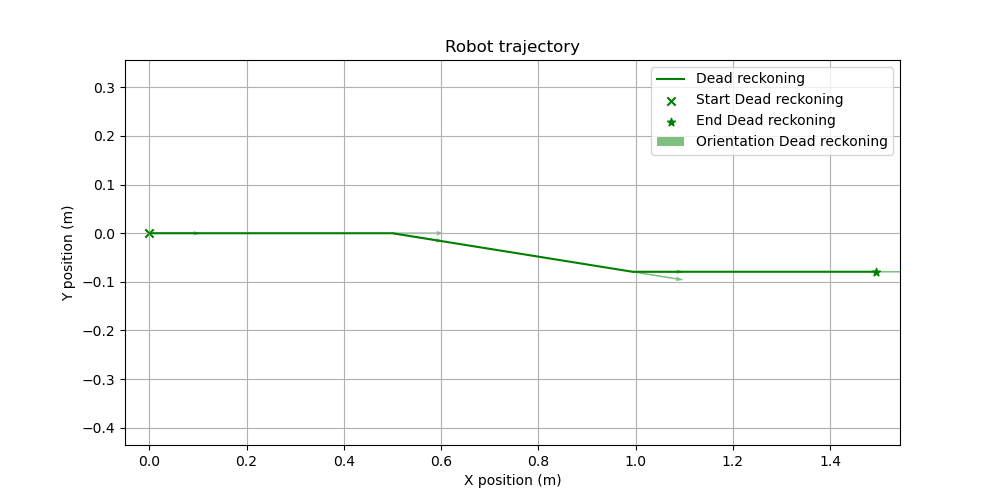
\includegraphics[width=\textwidth]{Figure_1.png}
\caption{Robot motion model test on example commands}
\end{figure}

\subsection{Motion model test on robot dataset}
The starting point of the dead-reckoned path uses the ground truth for its initial state. We can observe a growing drift that is only additive. The trajectory loosely tracks for a couple turns until it completely diverges.
% find where divergence starts and why
% show error plot

\begin{figure}
\centering
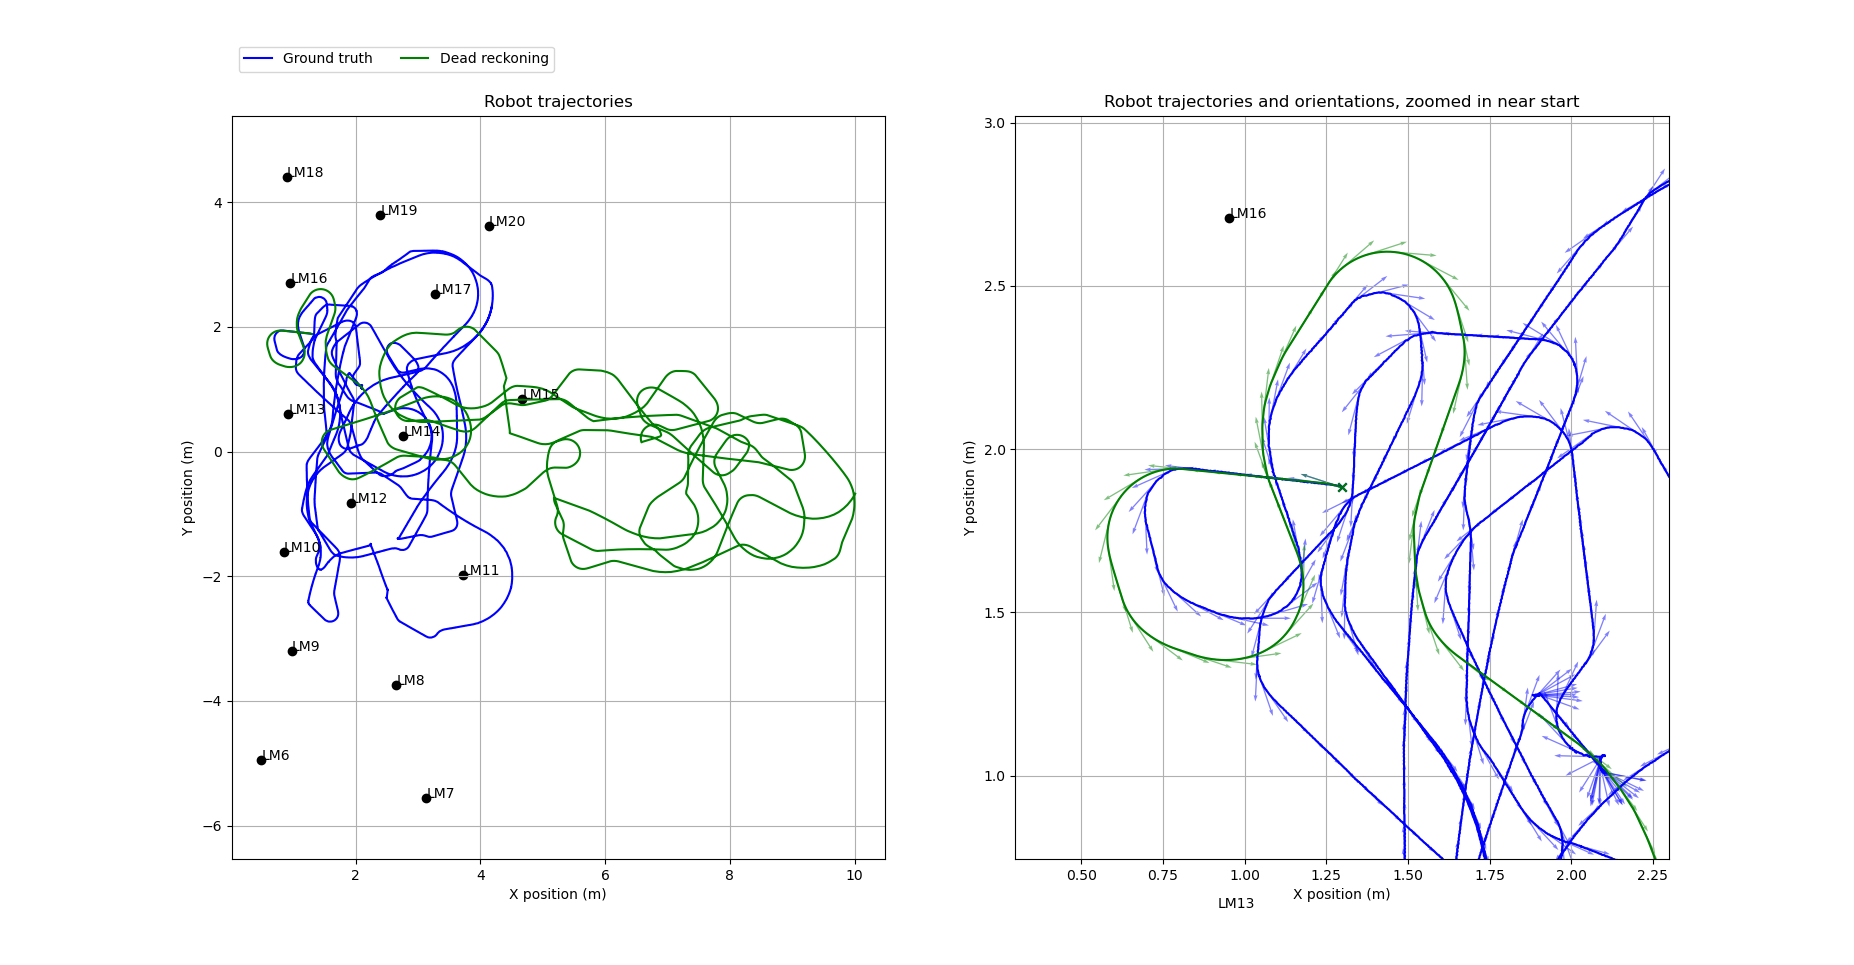
\includegraphics[width=\textwidth]{Figure_2.png}
\caption{Robot dead reckoning, compared to ground truth}
\end{figure}

\begin{figure}
\centering
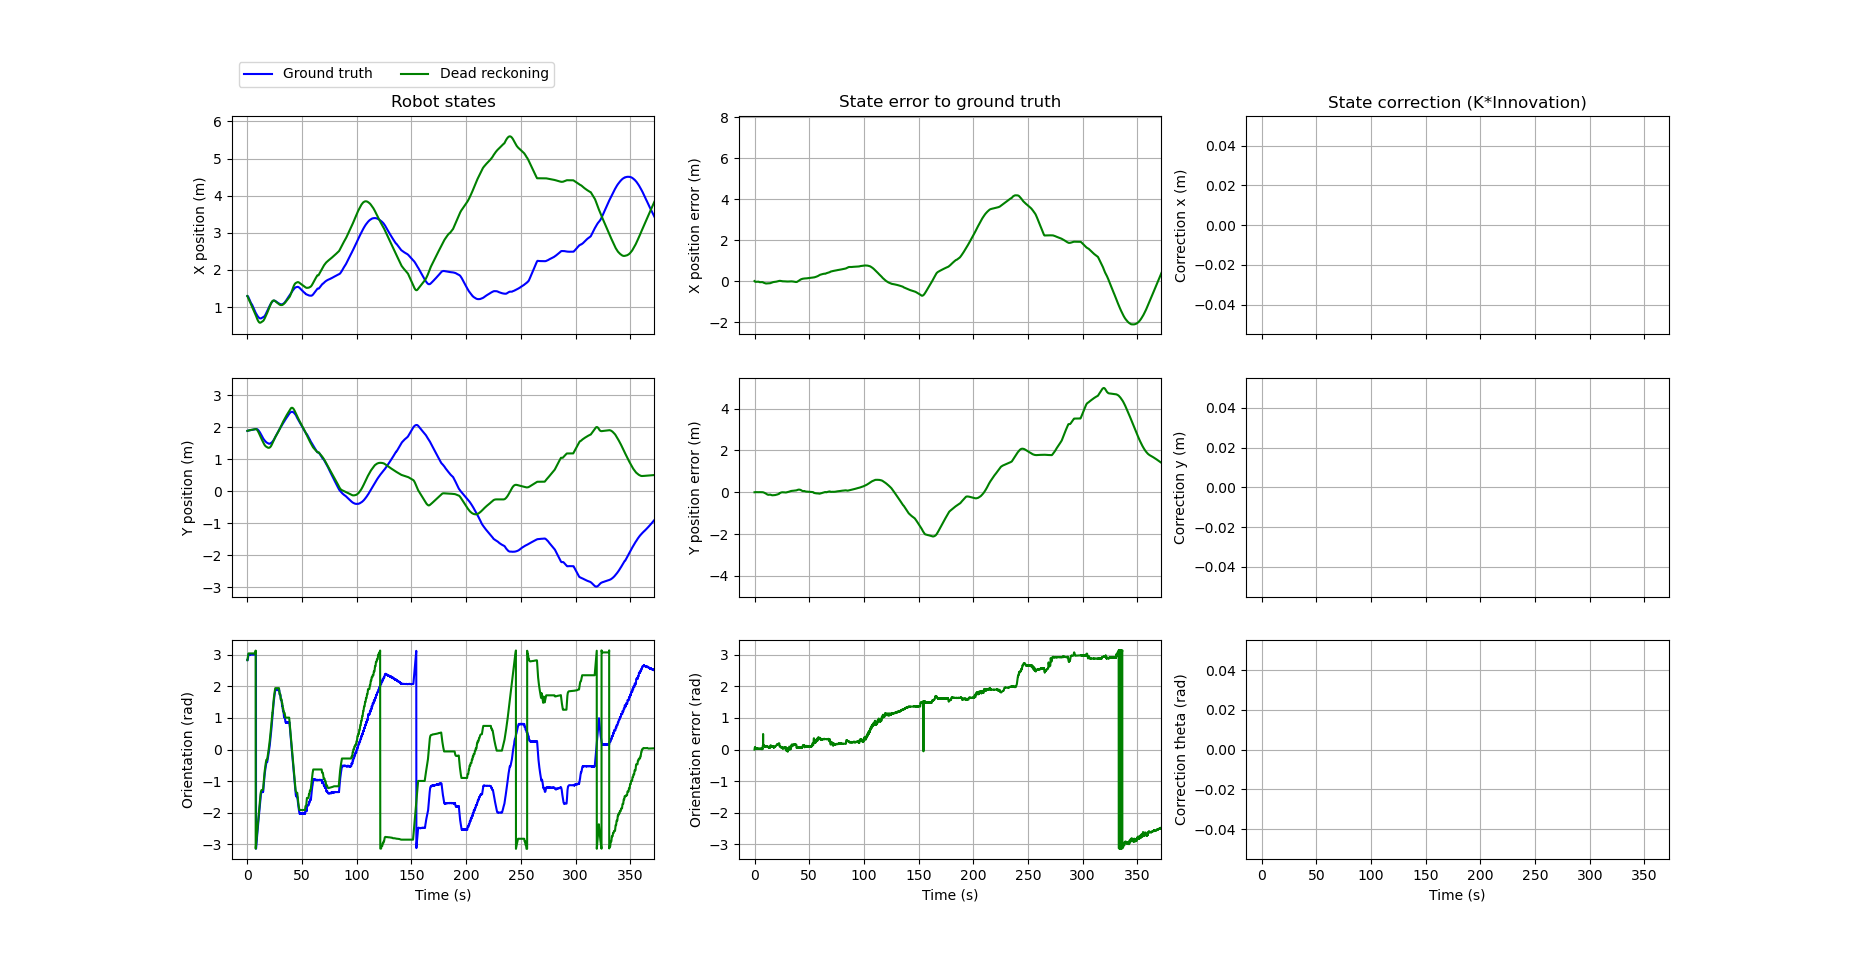
\includegraphics[width=\textwidth]{Figure_3.png}
\caption{Robot position and error}
\end{figure}

\subsection{Unscented Kalman Filter}

An unscented Kalman filter (UKF) is fundamentally identical to a Kalman filter, in that unfolds in two steps. The first step is the prediction: it estimates a posterior belief by means of a motion model based on prior state and a control command applied over a time step. The second step is the correction: it uses a measurement model to create an expected measurement of that posterior belief. This is then compared to the actual measurement, and the posterior belief is adjusted based on the difference between expected and actual measurement. Some knowledge of the uncertainty of both model is required for this correction step.

The UKF is different in that it is meant for non-linear models, where the state uncertainty probabilistic parametrisation (gaussian) is not conserved through the model. Instead, the uncertainty is propagated by evaluating sample points (sigma points) through the motion model, and a mean belief and associated covariance is recreated from those points. New sigma points are generated to pass through the measurement model and a mean measurement and associated covariance are constructed. 
% add sigma point math
The remaining algebraic operations are performed on those means (posterior belief and measurement belief).
% Add matric math here


\subsection{Measurement model}

The measurement model takes the predicted belief $(x, y, \theta)$ as input as well as knowledge about the space, in this case the measured (assumed true) positions of the landmarks (those are available via the Landmark Groundtruth file).
The model outputs an estimated measurement range and bearing.

The derivation of the measurement model is as follows:
% add math equations and drawing

The measurement data reads landmark barcodes. Those need to be converted to the subject number between 6 and 20 so that they can be paired with the ground truth landmark data. This is done using the barcodes file.


\subsection{Test of measurement model on robot data}
The measurement model contains no noise and the positions provided are assumed to be the known robot position. The measurement model successfully finds all landmarks with zero error.


\section{Part B}
\subsection{Filter implementation}

In order for the filter to be implemented on this dataset, some attention needs to be paid to synchronize the data. The controls and the measurements are on different time grids. We interpolate the controls data over a fixed timestep chosen to be 0.05. This timestep can be updated but seems to have little effects on the overall behavior. The measurements are grounped to the nearest timestep. Because of the lower accuracy of those measurement, this will prove acceptable.

Special attention also needs to be paid when working with angle. Anytime an angle is manipulated, we will normalize it between $]-\pi,\pi]$ and we will use the circular mean to compute means.
% add ref to wiki


\subsection{Comparison to dead reckoning}
The commands from step 2 lead to similar results for both model, if the process noise covariance has a high impact on the motion model.
Let us looks at the data and try to undestand the order of magnitude of the covariance matrices.
Looking at the control data set (resampled at 0.05s intervals), the we find $\nu<0.1m/s$ and $\omega<0.6rad/s$. This means the order of magnitude of the state will evolve after a timestep is ($0.005m$ and $0.03rad$). If the standard deviation is of that magnitude, (covariance $\sigma_x=\sigma_y=0.00025,\sigma_\theta=0.001$), we can expect significan noise and non realistic posterior updates. 
We don't expect the motion model to be an order of magnitude off, it is reasonable to set the process noise covariance matrix an order of magnitude below.
We have no data on the measurements accuracy or the robot sensor.

% review values for example
We will assume moving forward that the process noise covariance is set to appropriate values as explained above (and more will be discussed below when reviewing parameter tuning).
Now looking at the robot dataset, we can find that the first measurement is collected at $t=11.100s$. Until then, both model match (prediction step only, no correction).
% observations prior to DR diverging
% drift triggered by event

\begin{figure}
\centering
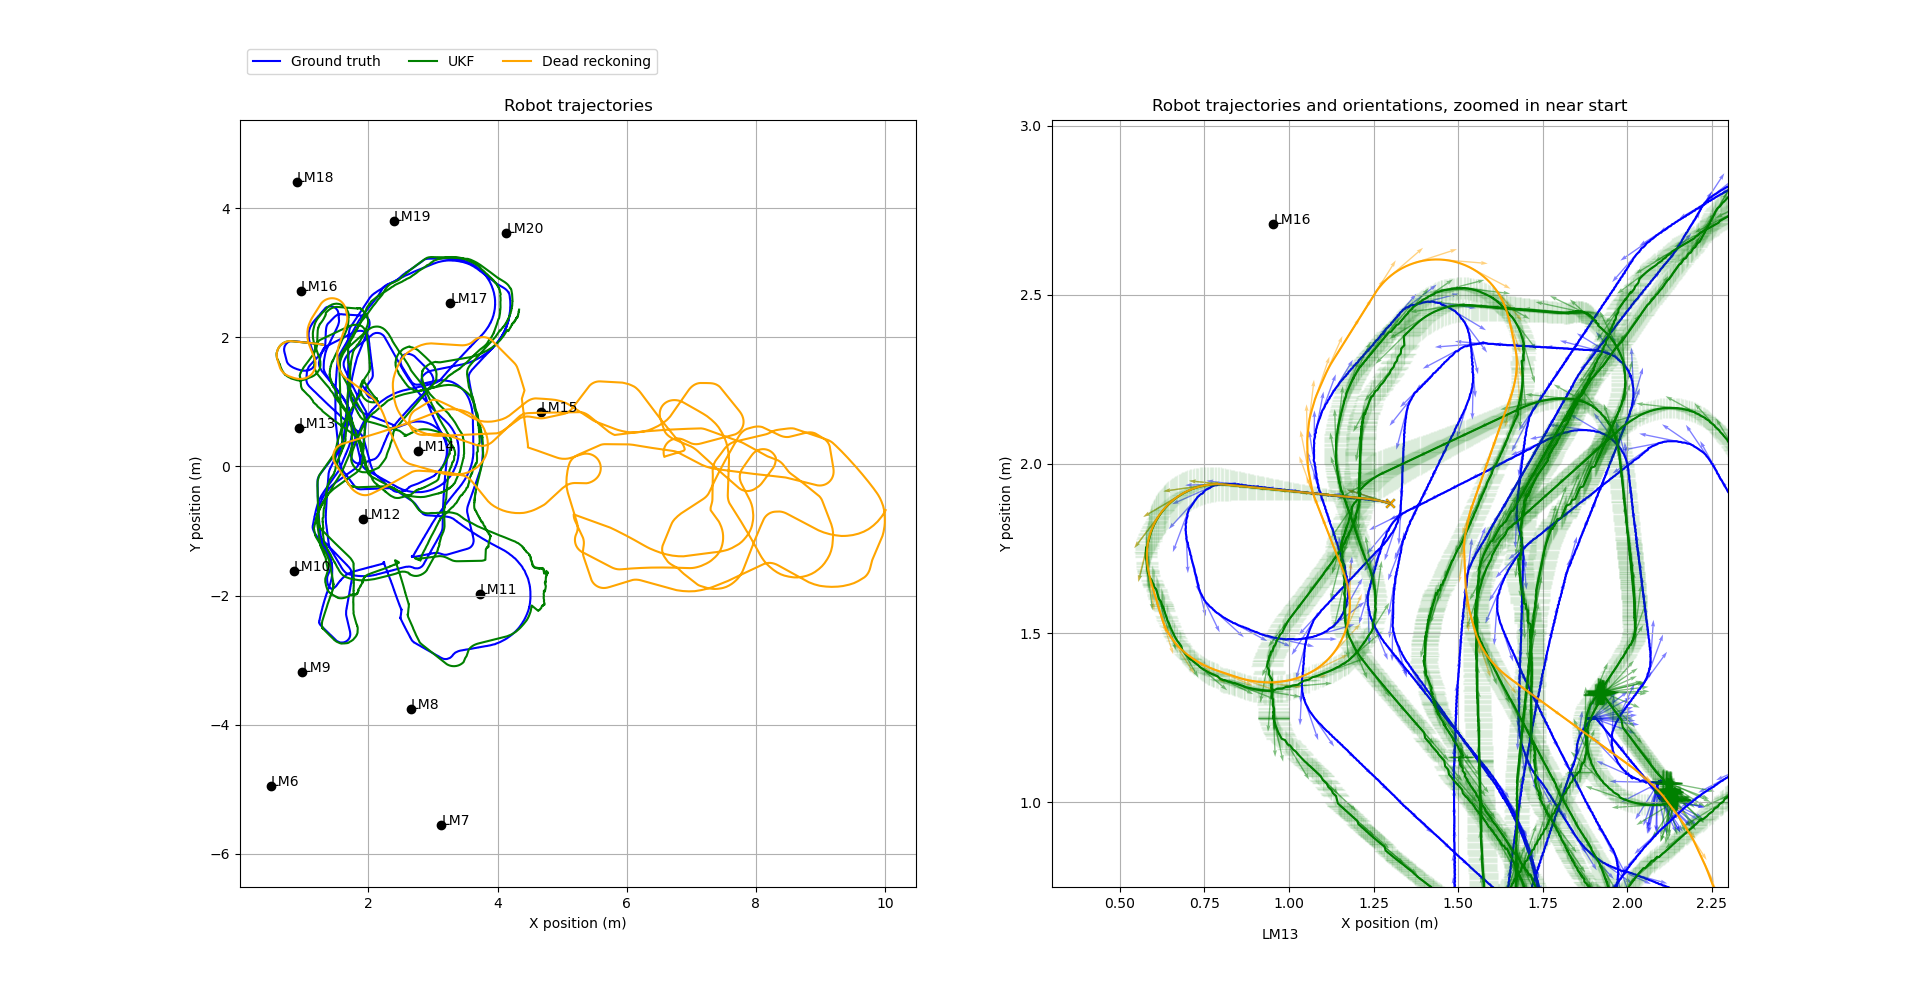
\includegraphics[width=\textwidth]{Figure_4.png}
\caption{Robot trajectory predictions with and without UKF}
\end{figure}


\begin{figure}
\centering
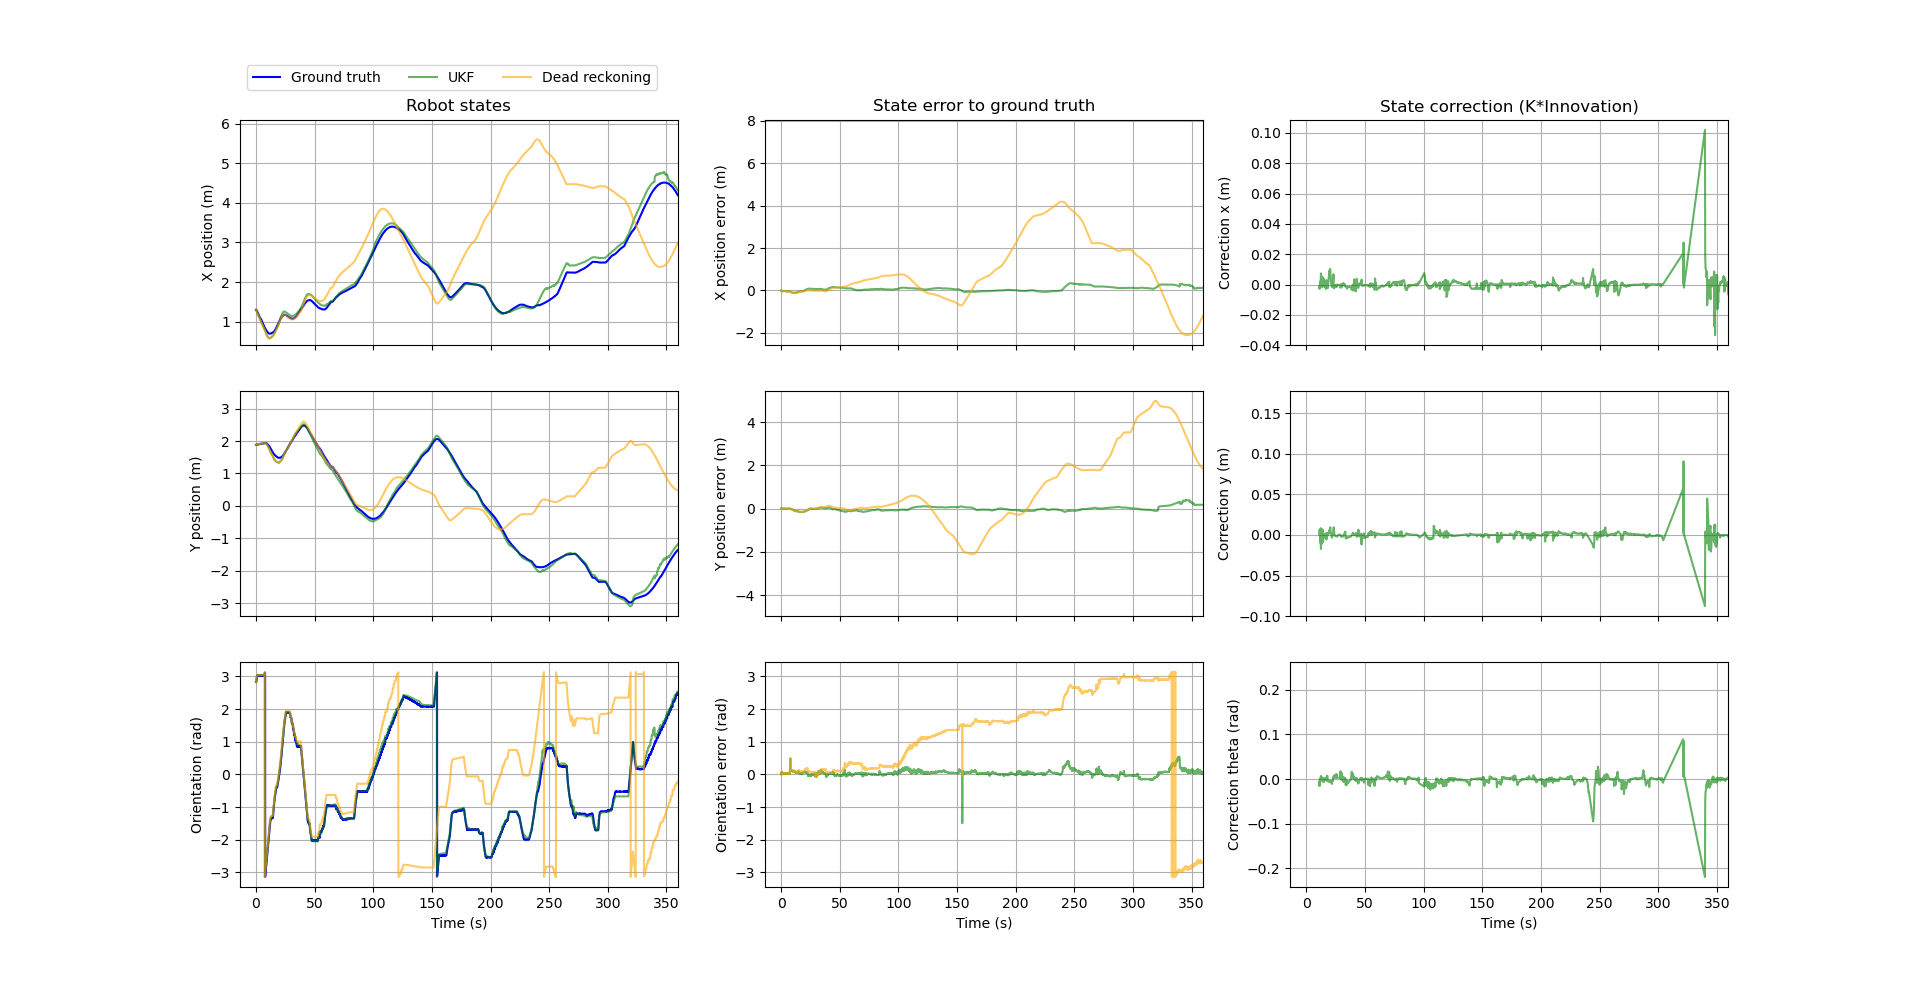
\includegraphics[width=\textwidth]{Figure_5.png}
\caption{Robot states and errors}
\end{figure}

\subsection{Filter analysis}
We will in this section perform an exploration of the different filter parameters.
The following assumptions have been made for simplicity:
- x and y have the same covariances. 
- $\theta$ covariance
- range and bearing
- the covariance matrices is diagonal, i.e. independence of the different state/measurement variables. 
- the initial state and its covariance, we use the ground truth to set the robot position. A very small initial state covariance makes sense. We will later look at this assumption and whether offseting the starting position impacts the model.

We have limited data available on the robot and its controls and sensors, the different covariance matrices (initial state covariance, process noise covariance and measurement noise covariance) have been assumed as diagonal elements of equal variances. An exploration in search of finding optimal parameters and understanding plausible assumptions is shown below. 
% review noise assumptions


\subsubsection{Process and measurement noise covariance}
Setting the process and measurement noise covariance is an iterative process. There is limited knowledge on the sensors being used on the robot. The motion model seems reasonable for short timesteps, especially if no differencial is applied from the controls (motion in straight line). We can get an idea of the standard deviation by looking at the dead reckoning model and estimating the drift over time.
% add plot drift between t=0-20
A starting point of $q=1e-6$ seems reasonable.
An estimation of the measurement noise covariance can be estalish iteratively. We will try $r=[1e-2, 1e-4, 1e-6, 1e-8]$.
The difference between the noise covariance matrices has a strong impact on the result. A smaller process noise covariance compared to the measurement one means that the posterior is more heavily influenced by the prediction step than the correction step (small Kalman gain * innovation). And vice versa.

A measurement noise covariance of 5 or more order of magnitude higher than the process noise covariance essentially leads the model to ignore the measurements and leaves the robot dead reckoning.
% plot dead reckoning and high r

A measurement noise covariance of the same magnitude as the process noise covariance leads to high overcorrection and very noisy posterior predictions: the position never stabilizes and drifts away from the ground truth. The state is updated with an equivalent control*dt that shows displacement beyond what can be expected reasonable (>10x expected motion).
% plot low r, show dt*control equivalent

It seems that a difference in order of magnitude of 4 leads to appreciable results. One can observe that shifting both the noise covariance higher or lower in pairs has little impact on the trajectory.
% plot shifting both in pairs

Plotting for process noise and measurement noise matched in pairs and offset by 4 orders of magnitude, one gets close to identical results (error within e-4 meters or 0.1mm). 4 OeM seems to lead to the smoothest trajectory (not over correcting) while minimizing error.

\begin{figure}
\centering
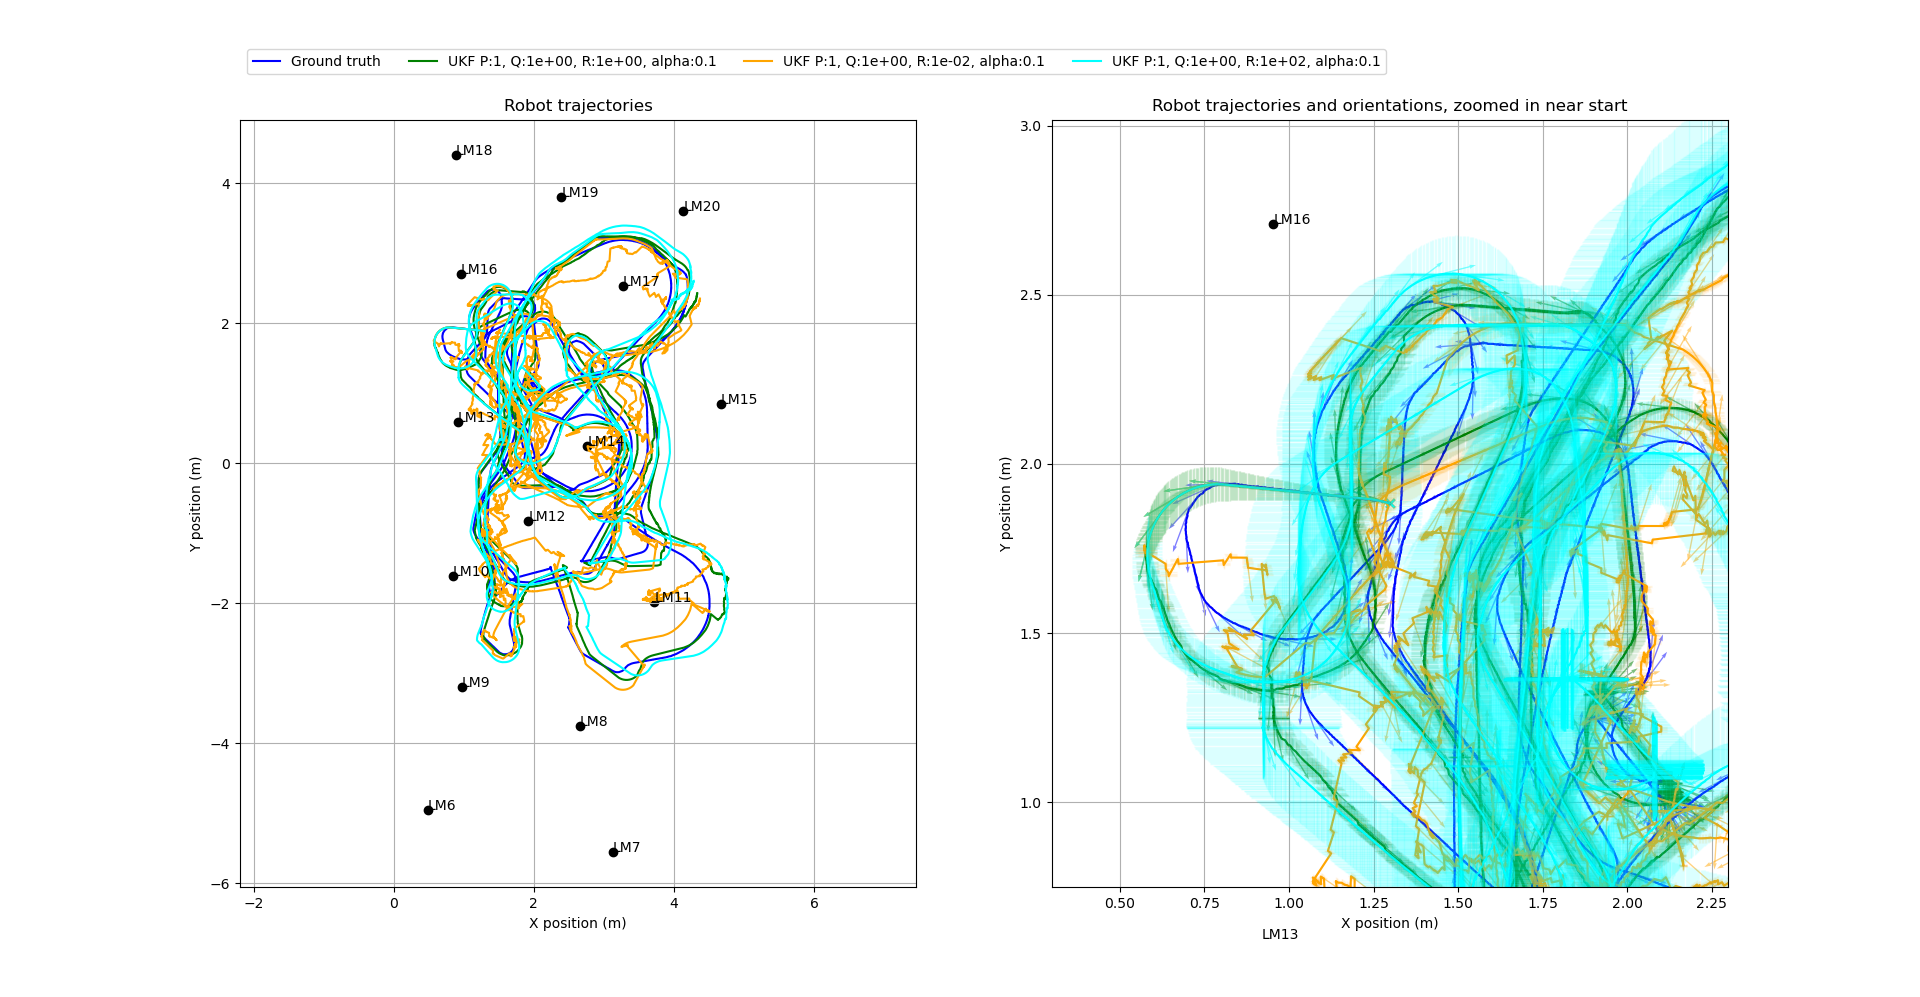
\includegraphics[width=\textwidth]{Figure_6.png}
\caption{Robot trajectory predictions for different UKF noise parameters. The 95 percent confidence interval on position is shown on the right figure.}
\end{figure}


\begin{figure}
\centering
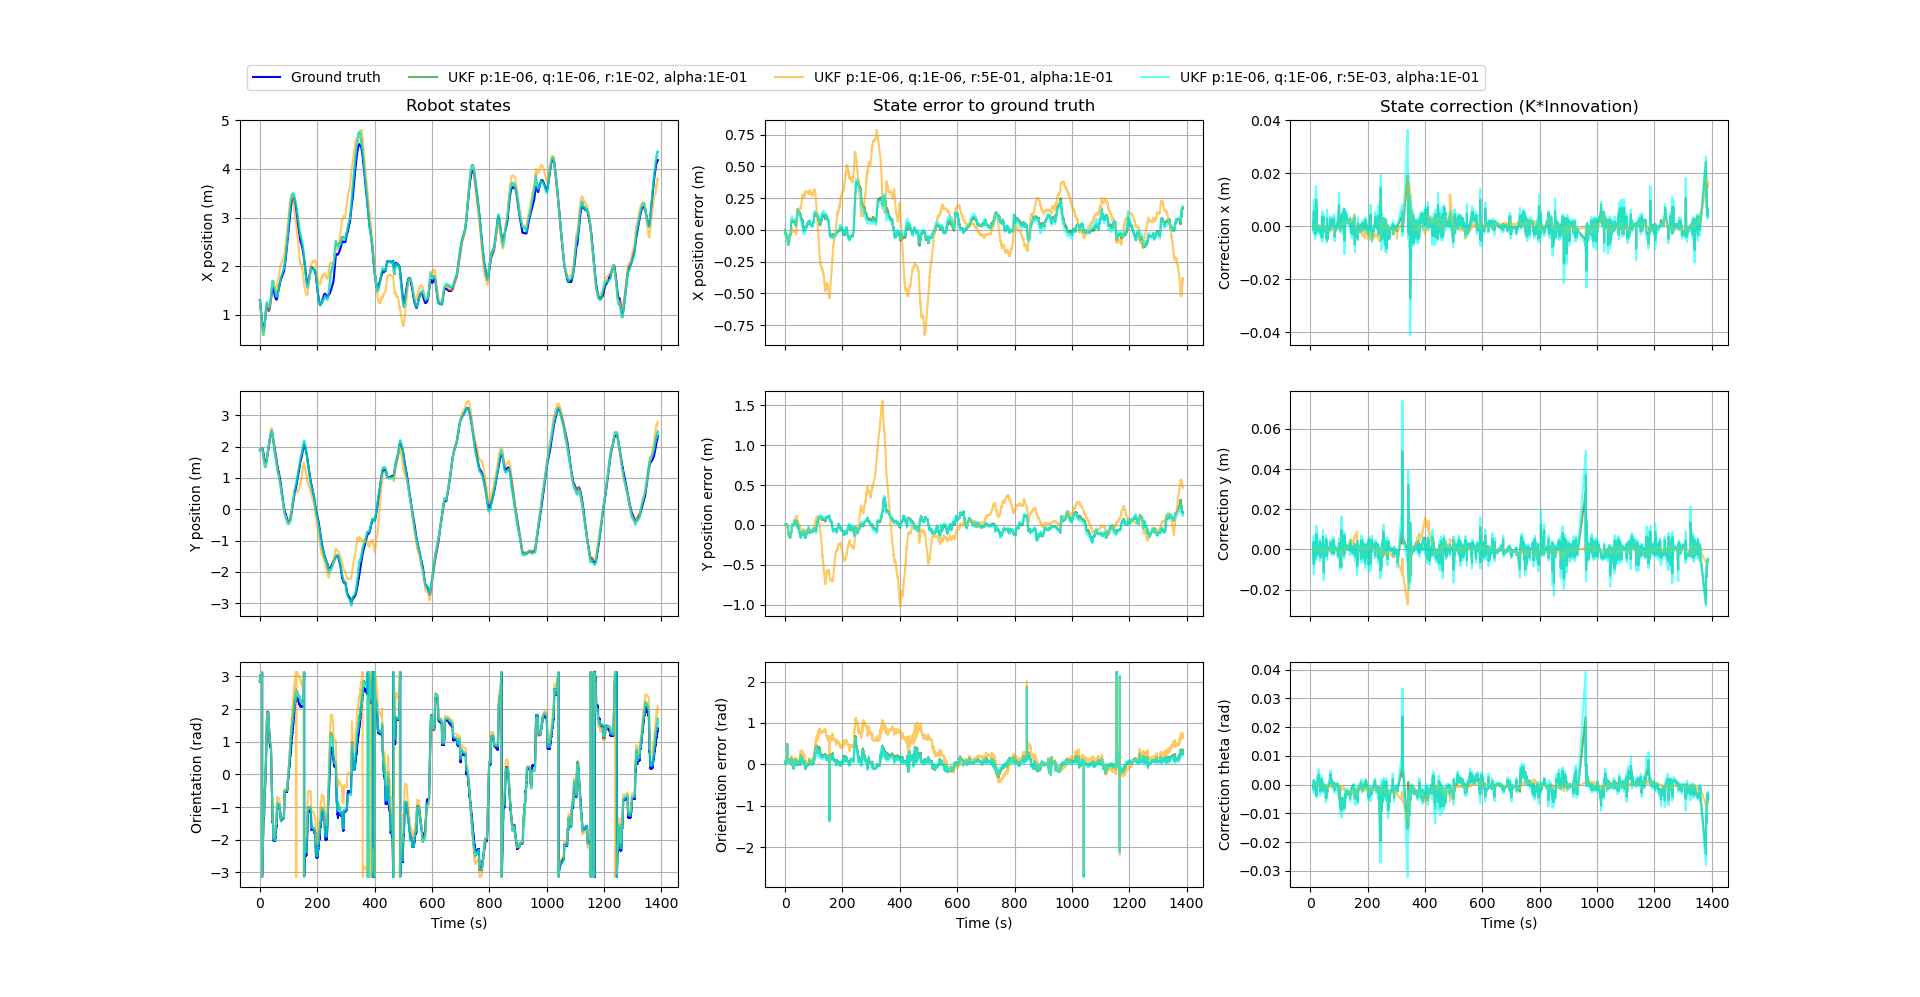
\includegraphics[width=\textwidth]{Figure_7.png}
\caption{Robot states and errors for different UKF noise parameters}
\end{figure}

\begin{figure}
\centering
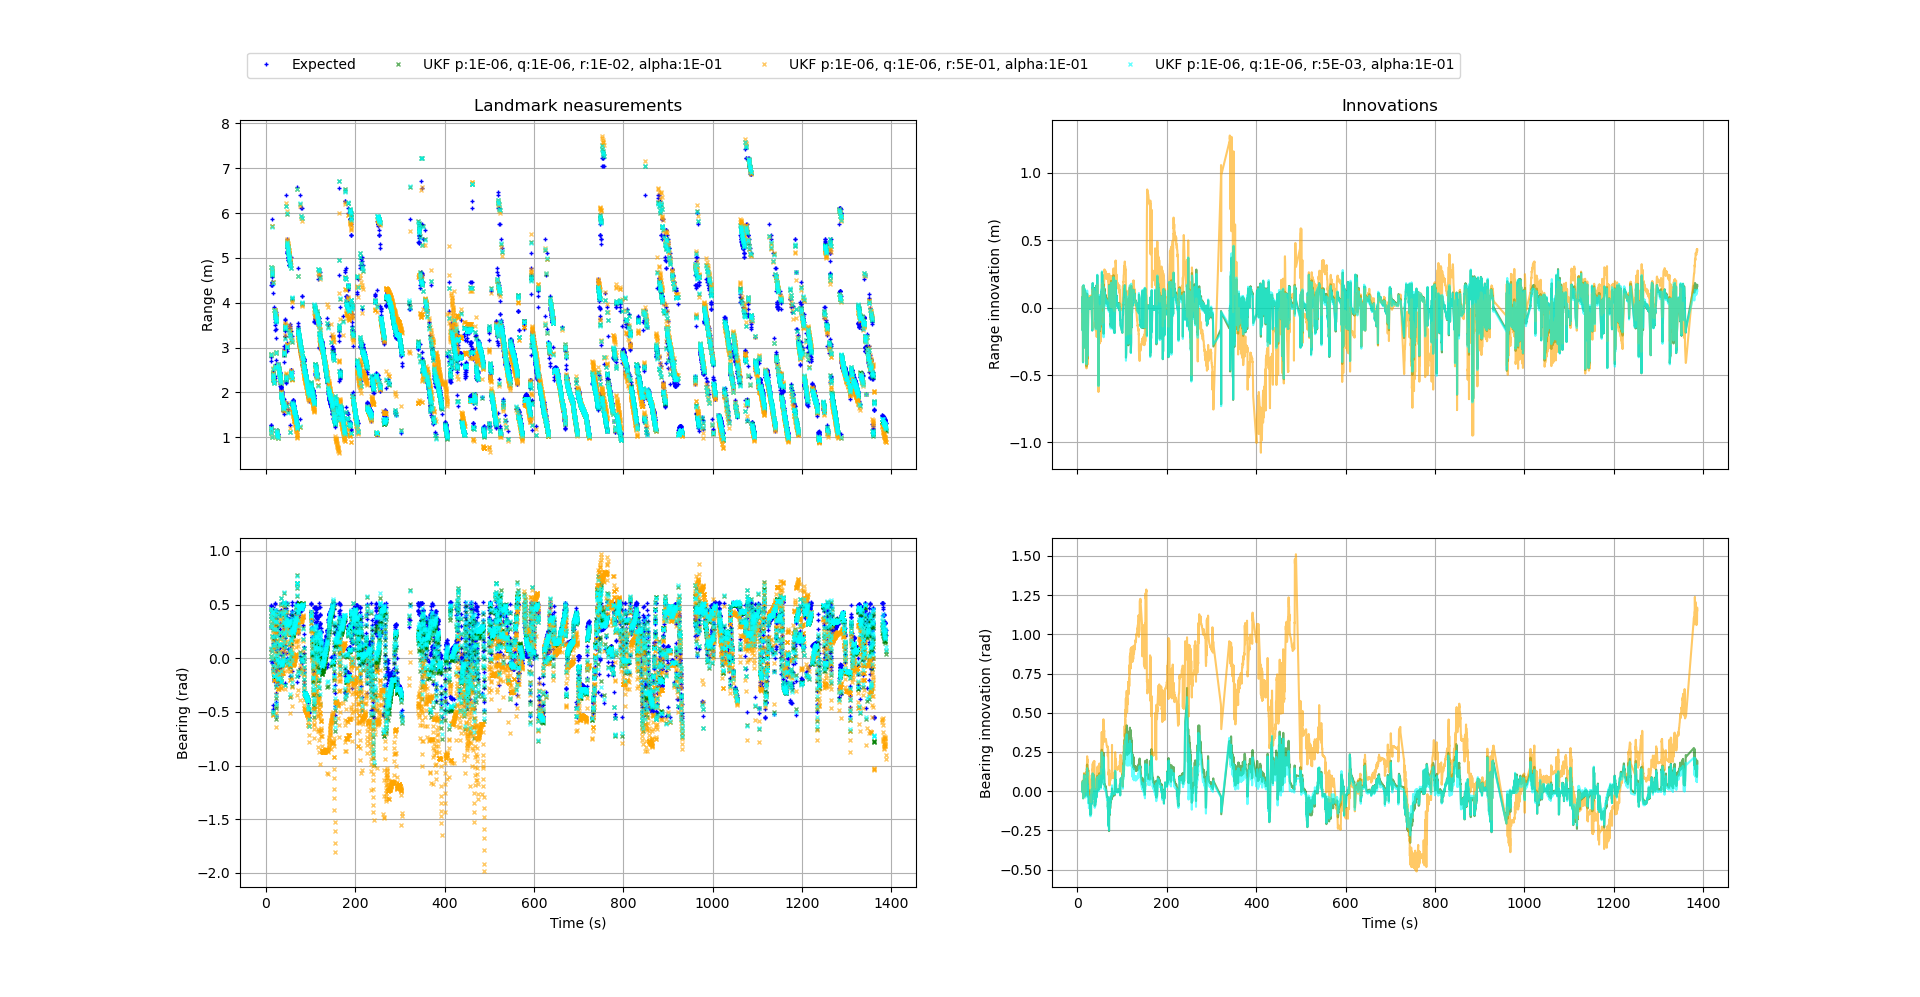
\includegraphics[width=\textwidth]{Figure_8.png}
\caption{Robot predicted measurements and innovations for different UKF noise parameters}
\end{figure}

\subsubsection{Initial state and its covariance}
For a known starting point, the initial state covariance has little to no impact.An initial covariance set fairly high (1e-1) will generate noise, this will however not last and the model corrects this behavior after a few seconds and all estimations become in agreement with one another.
% show plot with different initial cov
% move initial point and check impact on model

\subsubsection{Alpha}
Alpha controls the spread to the mean when creating the sigma points. After iteratiing for $\alpha=[0.01, 0.1, 1]$, it does not seem to have much of an impact on the behavior of the filter. This gives confidence in the capacity of the sigma points in capturing the non-linear behavior and the assumption about the state estimation as a gaussian.

\subsubsection{Missed measurement}
% find in data longest range with no measurement

\subsubsection{Multiple measurements}
% find litterature that suggest sequential correction (instead of weighted average)
If several measurements are found for a given time step, the correction step loops over the measurements one by one, using the corrected posterior as the new input for the next measurement.

\subsubsection{Final considerations}
A reminder in probability: the 95% confidence interval is given by +/-2*stddev, and the 99% confidence interface is given by +/-3*stddev.
The following parameters are eventually chosen:
$p=1e-6$ initial position.
$q=1e-6 (stddev=\sqrt(q)=0.001m or 1mm / 0.001rad or 0.06degrees)$ is a reasonable error assumption for a command over small dt (0.05s). 
$r=1e-2 (stddev=sqrt(r)=0.1m or 100mm / 0.1rad or 6degress)$ is a large but plausible error for the measurements.
$\alpha=0.1$ Alpha has been found to have little impact on this model and dataset. 


\subsection{How to write Mathematics}

\LaTeX{} is great at typesetting mathematics. Let $X_1, X_2, \ldots, X_n$ be a sequence of independent and identically distributed random variables with $\text{E}[X_i] = \mu$ and $\text{Var}[X_i] = \sigma^2 < \infty$, and let
\[S_n = \frac{X_1 + X_2 + \cdots + X_n}{n}
      = \frac{1}{n}\sum_{i}^{n} X_i\]
denote their mean. Then as $n$ approaches infinity, the random variables $\sqrt{n}(S_n - \mu)$ converge in distribution to a normal $\mathcal{N}(0, \sigma^2)$.


% \bibliographystyle{alpha}
% \bibliography{sample}

\end{document}
